\documentclass[en,license=none]{../../../eplsummary}
\usepackage{../../../eplcode}

\usepackage{esdiff}

\hypertitle{Machine Learning : regression dimensionality reduction and data visualization}{7}{ELEC}{2870}
{Guillaume Derval\and Benoît Legat}
{Michel Verleysen and John Lee}

\section{Introduction}
\subsection{What is machine learning}

The role of machine learning is to build a machine that learns a model from the data.
In statistics, one often suppose that the data follows a certain distribution and try to approximate the value of those parameters.
On the other hand, in machine learning we try to make the least amount of assumption on the data
to let enough degrees of freedom for the machine to learn a good model.

Machine Learning can be decomposed in 5 steps,
only the last 3 are covered in this course:
\begin{enumerate}
  \item
    Preprocessing
  \item
    Feature generation
  \item
    Feature selection (Section~\ref{sec:featuresel})
  \item
    Model generation (Section~\ref{sec:modelgen})
  \item
    Validation
\end{enumerate}

\subsection{History}
\begin{center}
  \begin{tabular}{lll}
    1940--1965 & Hebb                                 & Biological learning rule\\
               & McCulloch \& Pitts                   & Binary decision units\\
               & Rosenblatt                           & Perceptron, learning\\
    1969       & Minsky \& Papert                     & Limits to Perceptron\\
    1974       & Werbos                               & Back-propagation\\
    1980s      & Hopfield                             & Recurrent networks\\
               & Parker, LeCun, Rumelhart, McClelland & Back-propagation\\
               & Kohonen                              & Self-Organizing Maps\\
    1990s      & Vapnik                               & Support Vector Machines\\
               & Many                                 & Feature selection, model selection, evaluation...
  \end{tabular}
\end{center}

\subsection{Curse of dimensionality}
We need at least as much examples (data) than dimension.
If we cut each dimension by $x$, you have $x^n$ data samples.
We need at least some data in each region.
It increases expenentially.
So we need feature selection !

All our algorithms are sensitive to this problem, just differently.

\subsection{Learning with a Teacher: Supervised learning}
Learning with a labelled set, i.e. input-output examples; see \cite[p.~64]{haykin2009neural}.

Examples:
\begin{itemize}
  \item Regression: function approximation.
  \item Classification: heteroassociation \cite[p.~68]{haykin2009neural}, pattern recognition \cite[p.~69]{haykin2009neural}..
\end{itemize}
Note that classification can be seen as a particular case of regression,
e.g. a regression with discrete ``height'' values.

\subsection{Learning without a Teacher}
No labelled set.
\subsubsection{Reinforcement Learning}
Learning with a critic and an environment; see \cite[p.~66]{haykin2009neural}.
The output of the learning machine is perceived by the environment.
The critic extracts the input vector $x$ and a \emph{primary reinforcement signal} from the environment
and gives to the learning system a \emph{heuristic reinforcement signal}.

The learning system have therefore an input vector from the environment and a heursitic reinforcement signal from the critic that is used in place of the know output of the labelled set to learn.

\subsubsection{Unsupervised Learning or self-organized learning}
No labelled set and no teacher; see \cite[p.~67]{haykin2009neural}.

\begin{itemize}
  \item Clustering: autoassociation \cite[p.~68]{haykin2009neural}
  \item Adaptative filtering.
  \item Visualization.
\end{itemize}

\section{Feature selection}
\label{sec:featuresel}
\subsection{Principal Component Analysis (PCA)}
Suppose the features are stored by columns (resp. by rows) in $X$
and each row (resp. column) represents a sample
\subsubsection{Background}
\begin{itemize}
\item \textbf{Decorellated}: Data $(X,Y)$ are decorellated iff $C_{X,Y}$ is in the form of $\begin{pmatrix}
   \sigma_X^2 & 0 \\
   0 & \sigma_Y^2
\end{pmatrix}$.
The correlation of $n$ variables is computed using $C_X = X^\Tr X$ (resp. $C_X = XX^\Tr$).
\item \textbf{Whiteness}: Data $(X,Y)$ is white iff $C_{X,Y}$ is the identity matrix and $\bar{X}=\bar{Y}=0$.
\item \textbf{EVD}: Let $V$ be the matrix whose the column contain the eigenvectors of $C_X$, we have $C_X = V \Lambda V^\Tr$.
\item \textbf{Decorellation}: Find a transformation $W$ such that $XW$ (resp. $WX$) is decorrelated.
  Works for $W = V$ (resp. $W = V^\Tr$).
\item \textbf{Whitening}: Find a transformation $W$ such that $XW$ (resp. $WX$) is white.
  Works for $W = V\Lambda^{-\frac{1}{2}}$ (resp. $W = \Lambda^{-\frac{1}{2}} V^\Tr$).
\end{itemize}
\subsubsection{PCA Axes}
\begin{itemize}
\item Find axes that maximise the variance after projection
\item Best choice at each step is the eigenvector with the maximum eigenvalue
\item \textbf{Variance kept}: sum of the eigenvalues taken / sum of all the eigenvalues
\item \textbf{Error}: sum of the eigenvalues not taken / sum of all the eigenvalues
\item \textbf{Whiteness invariance}: rotations are white too (rotation matrix $T$ is orthogonal)
\end{itemize}

\subsection{Independent Component Analysis (ICA)}
\begin{itemize}
\item \textbf{Make features independent}
\item \textbf{Independance} between $X,Y$: $E[f(X)g(Y)]=E[f(X)]E[g(X)] \forall\ f,g$, $P(X|Y)=P(X)P(Y)$
\item Try to find independent unknown signal $s(t)$ by applying a matrix $W$ to the measured signals $x(t)=As(t)$ ($A$ unknown). We must find $W\approx A^{-1}$.
\item \textbf{Hypothesis}: mixture linear and additive (matrix $A$), random variables are signals, no delays, $E[s_is_i^\Tr ]=1$, $A$ constant over time
\item To find $W$, we try to make $y=Wx$ independent.
\item \textbf{Indeterminacies}: order of signals, scaling factor
\item \textbf{Whitening}: whitening $x$ allows to reduces $W$ to an orthogonal matrix ($VA$ is orthogonal), reducing the number of parameters to $n(n-1)/2$ from $n^2$.
\end{itemize}
\subsubsection{Non-gaussian approach}
\begin{itemize}
\item PDF of a sum of $n$ independant random variables tends to be Gaussian
\item Try to find $W$ such that output of PDF are as different as possible from Gaussian
\item \textbf{Minimum differential entropy} Trying to minimise entropy of $y$
\item \textbf{Negentropy}: Difference of entropy with a gaussian: $J(x)=\int p_x(u)\log\frac{p_x(u)}{p_{x_G}(u)}\ du$. Maximise $J(y)$.
\item \textbf{Kurtosis}: $\kappa_4(X)=E[X^4]-3E[X^2]^2$. For Gaussian functions, $\kappa_4(X_G)=0$. For others, $\neq 0$. Try to maximise $\sum_{i=1}^m|\kappa_4(Y_i)|$.
\item \textbf{Gram-Charlier Expansion} approximate PDF around a gaussian PDF
\end{itemize}
\subsubsection{Minimum dependance approach}
\begin{itemize}
\item \textbf{Minimise mutual information} (need joint PDF)
\item \textbf{Minimise sum of entropy}
\end{itemize}
\subsubsection{Practice}
\begin{itemize}
\item We do not know PDF
\item Density estimation to approximate PDF
\item Direct estimation of the independance (cross-cumulants)
\end{itemize}



\subsection{Feature selection}
\begin{itemize}
\item Most of the data, we have lot of dimensions, and not enough data
\item Distance means ``nothing'' in high-dimensional data
\item \textbf{Reducing the dimensionality}
\end{itemize}

\subsubsection{Filters}
\begin{itemize}
\item Does not use models.
\item \textbf{Correlation}: $r=\frac{\sum_{j=1}^N((x_j-\bar{x})(y_j-\bar{y}))}{\sqrt{\sum_{j=1}^N((x_j-\bar{x})^2)\sum_{j=1}^N((y_j-\bar{y})^2)}}$

\item \textbf{Entropy}: measure of uncertainty of a random variable: $H(x) = -E[\log(P[x])]$.
\item \textbf{Mutual information}: $I(y;x) = H(y)-H(y|x)=H(x)-H(x|y)$
\item \textbf{Relevance}: $I(x_i,t)$ (trying to maximise)
\item \textbf{Redundancy}: $I(x_i,x_j)$ (trying to minimise)
\item \textbf{Multi-objective optimisation}
\end{itemize}
\subsubsection{Wrappers}
\begin{itemize}
\item Uses models (select features that makes the model behave better)
\item Slower than filters
\item Relevance criterion easy to estimate
\item Less intuitive than filters
\end{itemize}
\subsubsection{Greedy search method}
\begin{itemize}
\item Testing $2^d$ subset is too much
\item Be greedy
\item Initial subset, simple update strategy + stop strategy
\item \textbf{Forward search}: begin with the empty subset, add the best feature, then stop when it decreases the performance
\item \textbf{Backward search}: idem, but with all the features as initial subset, then remove features
\item \textbf{Forward-backward}: allow to add and remove variable
\item \textbf{Genetic algorithms}
\end{itemize}
\subsubsection{Embedded methods}
\begin{itemize}
\item Feature selection + Model selection together
\end{itemize}


\section{Model generation}
\label{sec:modelgen}
\subsection{Linear regression}
\begin{itemize}
\item \textbf{Main notation}: $y = w^\Tr x$, with $x=(1,x_1,x_2,...,x_N)^\Tr $ and $w=(w_0,w_1,w_2,...,w_N)^\Tr $.
\item \textbf{Error criterion (most common)}: $\frac{1}{P}\sum_{p=1}^P(t_p - w^\Tr x_p)^2=\frac{1}{P}\|t-w^\Tr X\|^2$
\end{itemize}
\subsubsection{Pseudo-inverse}
\begin{itemize}
\item \textbf{Derivative of error criterion}: $\diffp{E}{w}^\Tr = \frac{2}{P}(w^\Tr X-t^\Tr )X^\Tr $
\item \textbf{Minimum error at}: $w=(XX^\Tr )^{-1}Xt$
\end{itemize}
\subsubsection{Gradient descent}
\begin{itemize}
\item \textbf{Gradient descent}: $x(t+1) = x(t)-\alpha \diffp*{x}{t}{x(t)}$
\item \textbf{Gradient descent on error criterion}: $w(t+1) = w(t) - \frac{2\alpha}{P}X(t-X^\Tr w(t))$
\item \textbf{Stochastic gradient descent}: As we can write that $E=\frac{1}{P}\sum_{p=1}^PE_p$, we can optimize the $E_k$ one at a time. $w(t+1) = w(t) - \frac{2\alpha}{P}(t-x_k^\Tr w(t))x_k$
\end{itemize}
\subsubsection{Linear associative memory}
\begin{itemize}
\item Learning: $w=\sum_{p=1}^P t_px_p$.
\item Magic: iff $x$'s are orthogonal and normalized.
\end{itemize}
\subsubsection{Perceptron}
\begin{itemize}
\item With $sgn$ as activation function, classification model ($-1$ or $1$)
\item Object is correctly classified if $w^\Tr x_kt_k > 0$
\item \textbf{Ideal error criterion}: $E = -\sum_{w^\Tr x_kt_k < 0} 1$ (not continuous)
\item \textbf{Perceptron criterion}: $E = -\sum_{w^\Tr x_kt_k < 0} w^\Tr x_kt_k$ (continuous, but gradient is only piece-wise linear)
\item \textbf{Perceptron convergence theorem}: If a set is linearly separable, then gradient descent on the perceptron criterion will converge in a finite number of steps. Proof: verify that $\|w\|$ grows slower than $\sqrt{n}$ and that $w^\Tr_{SOL}w$ is bounded below by a linear function of $n$.
\end{itemize}
\subsection{Multi-layer perceptron}
\subsubsection{Single layer}
\begin{itemize}
\item \textbf{Activation function}: $\sigma(w^\Tr x)$
\item \textbf{Error function}: $E = \frac{1}{P}\sum_{p=1}^P(t_p - \sigma(w^\Tr x_p))^2$
\item \textbf{Stochastic gradient descent rule}: $w(t+1) = w(t) - \frac{2\alpha}{P}(t-x_k^\Tr w(t))x_k \diffp*{\sigma}{p}{w(t)^\Tr x_k}$
\end{itemize}
\subsubsection{Multi-layer}
\begin{itemize}
\item \textbf{Model}:  $y(x) = h(w^{(2)}g(w^{(1)}x))$, $h$ can be linear, but not $g$.
\item \textbf{Universal approximation property}: 2-layer MLP can approximate everything to an arbitrary precision if there are enough hidden units.
\item \textbf{Learning}: Algorithm
	\begin{enumerate}
		\item Apply an input vector $x_k$ through the network, computing all values
		\item Evaluate error  on the last layer (difference with $t_k$)
		\item Back-propagate the error on each layer
		\item Compute all the derivatives of $E$
		\item Gradient descent step
	\end{enumerate}
\end{itemize}
\subsubsection{Improvement to gradient descent}
\begin{itemize}
\item \textbf{Momentum}: add $\beta(w(t)-w(t-1))$ after the gradient descent step ($\beta\approx 0.9$)
\item \textbf{Adaptive learning rate}: making $\alpha$ a function, increasing (resp. decreasing) by a constant when the new direction is nearly the same as previous one (resp. not the same) (scalar product is $> 0$)
\end{itemize}
\subsubsection{Weight adjustment}
TODO

\subsection{Radial-basis function networks}
\begin{itemize}
\item \textbf{Cover's theorem}: The probability of $\phi$-separability ($\exists \textrm{ vector } w$ that linearly separates $\phi(X)$) tends to one if $\phi_i$ are not linear and more than the number of dimensions
\item \textbf{RBFN}: We search for $F:R_D\rightarrow R$ such that $F(x_p)=t_p \forall p \in P$. \\\
Solution (with regularization $\lambda$): $$F(x) = \sum_{p=1}^P w_pG(x,x_p)$$ $$w=(G+\lambda I)^{-1}t$$ ($G+\lambda I$ non-singular if $x_k$ distincts (Michelli)).
\item \textbf{Generalized RBFN}: $$F(x) = \sum_{i=1}^K w_p\phi(\|x-c_i\|)$$ $$\phi(\|x-c_i\|)=exp(-\frac{\|x-c_i\|^2}{2\sigma_i^2})$$
\item \textbf{Park \& Sandberg}: For any function $f$, it exists a function $F$ with an unspecified $K$ that approximates $f$ as good as willed.
\item \textbf{Learning}:
	\begin{enumerate}
		\item \textbf{Centers} $c_i$: use Vector quantization to find the centers ($c_i$ are centroids)
		\item \textbf{Widths} $\sigma_i$: choose them according to the standard deviation around the centroids
		\item \textbf{Weigths} $w_i$: with $c_i$ and $\sigma_i$, finding $w_i$ becomes linear. Simply use pseudo-inverse or SVD.
	\end{enumerate}
\item \textbf{Standard deviation of the widths}:
	\begin{itemize}
		\item $\sigma = \frac{d_{max}}{\sqrt{2K}}$ where $d_{max}$ is the max distance between centroids
		\item $\sigma_i = \frac{1}{q}\sqrt{\sum_{j=1}{q}\|c_i-c_j\|^2}$ scan the $q$ nearest centroids
		\item $\sigma_i = r \min_j(\|c_i-c_j\|)$ where $r$ is an overlap constant
	\end{itemize}
\item \textbf{Improvements}:
	\begin{itemize}
		\item Optionnal computation step: gradient descent on all parameters
		\item Add constant and linear terms to $F(x)$
		\item Normalize the $\phi_i$ to make them bounded to $[0,1]$
	\end{itemize}
\end{itemize}

\subsection{Vector Quantization}
\subsubsection{Background}
\begin{itemize}
\item \textbf{Goal}: find $Q$ vectors(\textbf{centroids}) ($Q<P$), simplifying the database, while minimizing the loss of information.
\item \textbf{Voronoi zone} (around a centroid): Subset of the space that lies closer to this centroid than to any other.
\item \textbf{Minkowski’s $L_P$ norm} $d_p(x_i,y_j) = (\sum_{k=1}^D x_{i,k}^p - y_{j,k}^p)^{1/p}$
\item \textbf{Euclidian distance} $d_2$ -> least square error.
\item \textbf{Weighted distances} $d_W(x_i,y_i) = (x_i-y_i)^\Tr W(x_i-y_i)$.
	\begin{itemize}
		\item \textbf{Mahalanobis distance} $W=C_{XY}$
		\item  \textbf{$W$ symmetrical} $d_W(x_i,y_j) = d_2(Px_i,Py_j)$ with $W=P^\Tr P$
	\end{itemize}
\end{itemize}
\subsubsection{Lloyd's principle}
\begin{itemize}
\item \textbf{Lloyd's Principle} VQ is a two stage process: $x_i \rightarrow \text{encoder } \alpha \rightarrow j \rightarrow \text{decoder } \beta \rightarrow y_j$.
\item \textbf{$\alpha$ known}: $\beta(j) = argmin_{y_j}(E(d(x_i,y_j)|\alpha(x^i)=j))$ (center of mass)
\item \textbf{$\beta$ known}: $\alpha(x_i) =  argmin_j(d(x_i,y_j)) \text{ where } y_j =\beta(j)$ (nearest neighbour)
\item \textbf{Lloyd's algorithm}
	\begin{enumerate}
		\item Choice initial centroids
		\item Evaluate current Error
		\item If Error small enough, stop
		\item Replace all centroids $y_j$ with the center-of-mass of the values associated to it
		\item Go back to step 2
	\end{enumerate}
	\begin{itemize}
		\item \textbf{Hypothesis}: Probability of finding a point on the border of a voronoi zone is $0$
		\item \textbf{Limitation}: Local minimum of the error
	\end{itemize}
\item \textbf{Initialisation of Lloyd's algo}:
	\begin{itemize}
		\item At random in the input space (no data taken into account)
		\item First $Q$ points of $X$
		\item Randomly chosen points in $X$
		\item Product codes: product of scalar quantizers
		\item Growing initial set (choose randomly in $X$, but keep only if distance is sufficient)
		\item Pairwise nearest neighbor (begin with all $X$, and at each step merge the two closest centroids). Variant: merge the two centroids giving the lowest increase of error.
		\item Splitting: Begin with two centroids, apply Lloyd's, then disturb them with two new, etc.
	\end{itemize}
\end{itemize}
\subsubsection{Competitive learning}
\begin{itemize}
	\item For each $x_i$, change the position of the nearest centroid: $y_k(t+1)=y_k(t)+\alpha(x_i-y_k)$
	\item $E = \int(x-y_{j(x)})^2p(x) dx$
	\item Robbins-Monro conditions on $\alpha$: $\sum_{t=0}^\infty \alpha(t) = \infty$ and $\sum_{t=0}^\infty \alpha(t)^2 < \infty$
	\item Local minima, lose centroids
	\item \textbf{Frequency-sensitive learning}: multiply the distances by a function $u$ that is incremented each time this centroid is selected
\end{itemize}
\subsubsection{Learning Vector Quantization}
\paragraph{LVQ1}
\begin{itemize}
\item With classes
\item Same algo as competitive learning if centroid and $x_i$ are in the same class: $y_k(t+1)=y_k(t)+\alpha(x_i-y_k)$
\item But increase distance of centroids of different classes than $x_i$: $y_k(t+1)=y_k(t)-\alpha(x_i-y_k)$
\end{itemize}
\paragraph{LVQ2}
\begin{itemize}
\item Try to reaches Bayes(optimal) boundary
\item Selection of two winners
\item Move the two winners if
	\begin{enumerate}
		\item One winner($y_{a}$) is in the same class as $x_i$ AND
		\item The other one($y_{b}$) is not AND
		\item $x_i$ is in between the two centroids, in a window of fixed size
	\end{enumerate}
\item Move: $y_a(t+1)=y_a(t)+\alpha(x_i-y_a(t))$ and $y_b(t+1)=y_b(t)+\alpha(x_i-y_b(t))$
\end{itemize}
\paragraph{Improvements}
\begin{itemize}
\item \textbf{Forgetting factor}: progressively ignore data for from boundary
\item \textbf{Dynamic Vector Quantization}: Add centroids if needed ($x_i$ of class 1 is the nearest point to centroid of class 2 or distance between point and centroid too wide)
\end{itemize}
\subsubsection{Winner-take-all/Winner-take-most}
\begin{itemize}
\item adapt the winner and other centroids as well
\item Example: \textbf{Neural gas}: add a factor $e^{-h(j,x_i)/\lambda}$ on the updates, where $h$ is the the number of the centroid when ordered by distance.
\end{itemize}

\subsection{Self-Organizing Maps}
\begin{itemize}
\item VQ with a supplementary grid space
\item \textbf{Topology conservation}: if centroids lie closely in the grid space, they are more likely to lie closely in data space
\item \textbf{Adaptation of weights}: Take the winner $k=\text{argmax}_i(w_i^\Tr x)$ and update the weights: $$w_j(t+1)= w_j(t) + \alpha(t)(x-w_j(t))V(k,j)$$
\item $\alpha(t)$ and $r(t)$ decrease over time.
\item $\alpha$ must follow Robbins-Monro conditions
\item \textbf{Hard neighbourhood}: $$V(k,j)=\left\{ \begin{array}{l l}
1 & \text{if} d(k,j)<r(t) \\
0 & \text{otherwise}
\end{array}
\right.$$
\item \textbf{Soft neighbourhood}: $V(k,j)=exp(-\frac{d^2(k,j)}{r^2(t)})$
\item \textbf{Butterfly effect}: If $r(t)$ decreases too fast with respect to $\alpha(t)$
\item \textbf{Pinch effect}: If $r(t)$ decreases too fast
\end{itemize}
\subsubsection{Measures of quality}
\begin{itemize}
\item \textbf{Quality of VQ}: use VQ techniques
\item \textbf{Quality of Organization}: $dw-dr$
\item $dw$: distance of centroids in weight space
\item $dr$: distance between centroids in grid space
\item $dw-dr$: should be a straight line
\end{itemize}



\subsection{Support Vector Machines}
\subsubsection{Linear}
\begin{itemize}
\item Decision surface: hyperplane
\item Tries to maximise margin
\item \textbf{Hard-margin} Find $w,b$ such that $\|w\|^2$ is minimised and $y_i(w^\Tr x_i+b)\geq 1, \forall x_i$. Quadratic, convex, simple to compute
\item \textbf{Soft-margin} Allow errors, but penalize them with a parameter $C$. Constraint: $y_i(w^\Tr x_i+b)\geq 1-\epsilon_i, \forall x_i$, with $\epsilon_i$ the (positive) error. Trying to minimise $\|w\|^2+C\sum_i\epsilon_i$.
\item Minimizing the number of misclassification is NP-complete
\end{itemize}
\subsubsection{Non-linear with Kernel trick}
\begin{itemize}
\item We try to find a map $\Phi(x)$ to allow to find non-linear surfaces: $y_i(w^\Tr \Phi(x_i)+b)\geq \epsilon_i, \forall x_i$
\item \textbf{Dual of the problem}:
$$\min_{\alpha_i}\frac{1}{2}\sum_{i,j}\alpha_i\alpha_jt_it_j(\Phi(x_i)^\Tr \Phi(x_j))-\sum_i\alpha_i$$
$$\text{s.t.} 0 \leq \alpha_i \leq C, \forall x_i$$
$$\sum_i \alpha_i t_i=0$$
\item \textbf{Kernel Trick}: We can find $K(x_i,x_j)=\Phi(x_i)^\Tr \Phi(x_j)$, that does the product without "directly" mapping
\item $\text{sgn}(w^\Tr \Phi(x)+b)=\text{sgn}(\sum_i\alpha_it_iK(x_i,x)+b)$ allows to classify
\item $b$ can be extracted by solving $\alpha_j(t_j\sum_i\alpha_it_iK(x_i,x_j)+b-1)=0 \text{ for a } j \text{ s.t. } \alpha_j \neq 0$
\end{itemize}
\subsubsection{Kernels}
\begin{itemize}
\item \textbf{Polynomial kernel of degree $p$}: $K(x,z)=(x^\Tr z+1)^p$
\item \textbf{Gaussian kernel}: $K(x,z)=exp(-\frac{\|x-z\|}{2\sigma^2})$ (parameter $\sigma$)
\item \textbf{Kernels must be symmetric}
\item \textbf{Any symmetric function does not involves the existence of an associated mapping}
\item \textbf{Gram matrix}: matrix where $G_{ij}=K(x_i,x_j)$
\item \textbf{Mercer condition}: a mapping $\Phi(x)$ exists when $G$ is semi-positive definite
\end{itemize}
\subsubsection{Comparison with MLP}
\begin{tabular}{l|l|l}
& MLP & SVM \\
\hline
Mapping to & Moderate dimensional space & Very high dimensional space \\
Unique minimum? & No & Yes \\
Training & Expensive & Efficient \\
Classification & Efficient & Efficient \\
(Hyper-)parameters & Number of hidden layers, units & kernel, kernel hp, $C$\\
Robust & Moderately & Yes
\end{tabular}




\section{Model Selection}

For the feature selection and model generation,
we often need to choose a few parameters,
e.g. the number of features, the number of neurons, ...

This parameter often changes the \emph{complexity} of the model.
As can be seen in \figuref{biasvariancecompromise}, increasing the model complexity
obviously enables the model to decrease the error on the learning set.
However, allowing the model to fit too much the data will allow it to start fitting the noise !
This decrease its ability to generalize.
In \figuref{biasvariancecompromise}, we see that the error on the validation set increase for a highly complex model.
This phenomemon is called overfitting.

If our model is not complex enough, it might miss relevant relations between features and the output,
this is called underfitting.
The goal of model selection is to find the compromise between underfitting and overfitting.

\paragraph{Remark}
Increasing the size of the learning set decreases the risk of overfitting.

\begin{myfig}{biasvariancecompromise}{Model structure selection is a compromise between bias and variance}
  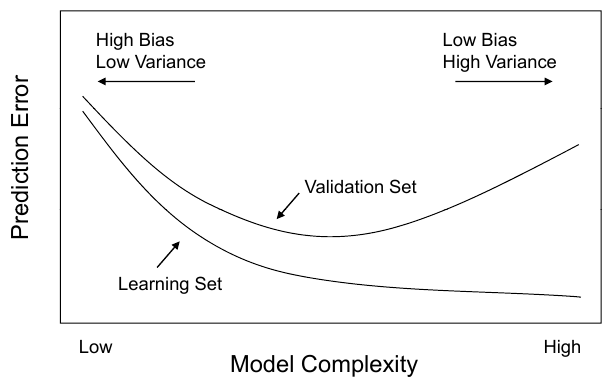
\includegraphics[width=0.6\textwidth]{biasvariancecompromise.png}
\end{myfig}

Different approaches exist for finding this compromise.
For each of them, the set used for learning is reduced
so we have even less data to find the value of the parameters of our model.
This is the price to pay to avoid overfitting.

%\subsubsection{2 different models}
%A solution is to take different parametric models.
%We take 2 sets of example,
%one to build the model and one to evaluate the model.
%We process the model (value of the parameters) for each model and evaluate
%them with the other set.

\subsection{Minimum-Description-Length principle}
The minimum-description-length (MDL) principle \cite[Section~2.6]{haykin2009neural} was pioneered by Rissanen in 1978 \cite{rissanen1978modeling}.
His inspiration can be trace back to Kolmogorov complexity theory in 1965 \cite{kolmogorov1965three}:
\begin{center}
  \emph{The algorithmic (descriptive) complexity of a data sequence is the length of the shortest binary computer program that prints out the sequence and then halts}
\end{center}

Rissanen's MDL principle can be formulated as follows
\begin{center}
  \emph{Given a set of hypotheses, $\mathcal{H}$, and a data sequence $d$, we should try to find the particular hypothesis or some combination of hypotheses in $\mathcal{H}$, that compresses the data sequence the most}.
\end{center}


\begin{myexem}
  For instance, suppose we have need to find the weights $w$ that explains a data sequence $(x_1,y_1), \ldots, (x_n,y_n)$
  with the relation $y = w^\Tr x + \text{noise}$.

  We have
  \[ p_{W|Y,X}(w|y,x) = \frac{p_{Y|W,X}(y|w,x)p_{W}(w)}{p_Y(y)}. \]
  The MAP estimator consists in choosing $w$ that maximizes
  \[ p_{Y|W,X}(y|w,x)p_{W}(w). \]
  and the MLE estimator consists in choosing $w$ that maximizes
  \[ p_{Y|W,X}(y|w,x). \]

  Suppose we have two estimates candidate:
  \begin{itemize}
    \item an overfitting $w$ that has very high values of $w$ that compensates each other but that minimises very well the errors $|w^\Tr x_i - y_i|$,
    \item a reasonable $w$ with low values of $w$ that minimize quite well the errors $|w^\Tr x_i - y_i|$
  \end{itemize}

  Clearly the first one should be discarded because $w$ is very improbable, that is, $p_W(w)$ is very low.
  However, the MLE do not take this into account.

  As this examples shows, doing machine learning without model selection is like using an MLE estimator instead of a MAP estimator.

  Since $-\log$ is an decreasing function,
  the MAP minimizes
  \[ -\sum_{i = 1}^n \log(p_{Y|W,X}(y|w,x)) \log(p_{W}(w)) \]
  and the MLE minimizes
  \[ -\sum_{i = 1}^n \log(p_{Y|W,X}(y|w,x)). \]

  Using Shannon's entropy, we see that the MAP minimizes
  \[ H(Y|W,X) + H(W) \]
  while the MLE minimizes
  \[ H(Y|W,X). \]

  Suppose Alice and Bob both receives $x_i$'s but Alice also receives $y_i$ and want to tell to Bob what is $y_i$.
  Beforehand, they decide the value of $w$ hence Bob will be able to compute $w^\Tr x_i$ and Alice only has to transmit $y_i-w^\Tr x_i$ which needs much less bits than transmitting $y_i$.

  The MLE minimizes the number of bits needed to transmit $y$ and don't care about the number of bits that will be used to transmit $w$.
  On the other hand, the MAP minimizes the number of bits needed to transmit $y$ plus de number of bits needed to transmit $w$

  It is clear that the MLE will overfit.
  The parameter modeling the complexity of the MAP estimator is the variance of $w$.
  For instance, if we consider that $w$ follows an $n$ dimensional normal of variance $\infty$, then all values of $w$ requires the same number of bits to transmit and the MAP will overfit. This is the most complex model.
  However if we consider that $w$ follows an $n$ dimensional normal of variance, say, 1, then for the first estimate candidate (the one that overfits), since the $w$ is not very likely, we will need a lot of bits to transmit it
  while for the second estimate candidate we will need a lot less bits.
\end{myexem}

There are three approaches.

\subsubsection{Regularization}
One solution to avoid overfitting is to include a cost for high values of $w$.
That, we minimize
\[ E(w) + \lambda\|w\|^2. \]
This is called regularization.

Note that this corresponds to the MAP estimator in a Gaussian Environment \cite[Section~2.4]{haykin2009neural}.

\subsubsection{Akaike Information Criterion (AIC)}
Let $N$ be the number of samples and
\[ E_{\theta}(x) = \frac{1}{N} \sum_{t=1}^N (g(x_t, \theta) - y_t)^2. \]
We denote by $\dim(\theta)$ the dimension of $\theta$,
that is, the number of parameters.
For instance, if $\theta = w \in \R^n$, then $\dim(\theta) = n$.

In 1973, Akaike proposed to approximate $H(W)$ with $\frac{2}{n} \dim(\theta)$ which gives the following generalization error:
\[ \hat{E}_{\text{gen}}(\theta) = E_\theta(X) + \frac{2}{N}\dim(\theta). \]

\subsubsection{Bayesian Information Criterion (BIC)/Minimum Description Length (MDL)}
In 1978, Rissanen proposed to approximate $H(W)$ with $\frac{\log(N)}{n} \dim(\theta)$ which gives the following generalization error:
\[ \hat{E}_{\text{gen}}(\theta) = E_\theta(X) + \frac{\ln(N)}{N}\dim(\theta). \]

\subsection{Validation}
\begin{itemize}
\item \textbf{Validation}: use a validation set
\item \textbf{Cross-validation}: repeat validations
\item \textbf{K-fold}: Divide in fold of fixed size $=N/K$. Learn with $K-1$ fold, test with the remaining one, then change the fold use to test, $K$ times.
\item \textbf{Leave-one-out}: K-fold with $K=N$.
\end{itemize}

\subsection{Bootstrap}
\begin{itemize}
\item \textbf{Plug-in principle}: use the empirical distribution of the parameter in a sample instead of the true distribution
\item \textbf{Notation $E_{A,B}$}: $A$ is the learning set, $B$ is the test set. $P$ is the real population, i.e. an hypothetic set of all the data possible,
  $S$ is the set used for learning.
\item \textbf{Bootstrap}: We want to approximate the error of our model on the real population ($E_{S,P}$). We try to find
  \[ \hat{E} = E_{S,P} = E_{S,P} + E_{S,S}-E_{S,S} = E_{S,S} + (E_{S,P}-E_{S,S}) \approx E_{S,S} + (E_{S^*,P^*}-E_{S^*,S^*}) \]
  where $E_{S^*,P^*}-E_{S^*,S^*}$ is called the optimism.
  We set $P^* = S$ and $S^*$ is a set of the same cardinality as $S$ where each element is picked at random in $S$ with replacement.
\item \textbf{Bootstrap .632}: Compute bootstrap replication with $P^* = S \setminus S^*$ instead of $P^* = S$ and use
  \[ \hat{E}=0.368 \cdot E_{S,S}+0.632 \cdot \hat{\text{optimism}}. \]
\end{itemize}
\subsection{Confusion Matrix}
\begin{itemize}
\item \textbf{Confusion matrix}: Matrix where entry $c_{ij}$ is the number of data of class $j$ that have been classified in $i$
\item \textbf{Bayes confusion matrix}: optimal confusion matrix using Bayes boundary
\end{itemize}

\subsection{Pruning}

\begin{itemize}
  \item \textbf{Direct pruning}: remove neurons/weight if it is not useful (output fixed, correlated with another, random,...). Dangerous.
  \item \textbf{Local least squares}: When removing a weight, compensate the difference by modifying the other weights.
\end{itemize}

\subsubsection{Optimal Brain Damage}
In 1989, Lecun et al. \cite{lecun1989optimal} introduce a method for choosing the weights to remove using the Hessian of the errors on the learning samples.

By Taylor expansion, for a change $\delta w$ on the weights, the corresponding $\delta E = E(w + \delta w) - E(w)$ is
\begin{align*}
  \delta E
  & = (\grad E)^\Tr \delta w + \frac{1}{2} (\delta w)^\Tr H (\delta w) + \bigoh(\|\delta w\|^3)\\
  & = (\grad E)^\Tr \delta w + \frac{1}{2} \left(\sum_{i=1}^n H_{ii}(\delta w_i)^2 + \sum_{i=1}^n\sum_{j=1}^n H_{ij} (\delta w_i) (\delta w_j) \right) + \bigoh(\|\delta w\|^3).
\end{align*}
where $\grad E$ is the gradient of $E$ at $w$ and $H$ is the hessian of $E$ at $w$.

After having trained the network, we know that $w$ is such that $(\grad E)^\Tr \delta w = 0$.
If we neglect $\bigoh(\|\delta w\|^3)$ we have
\begin{equation}
  \label{eq:Edw}
  \delta E \approx \frac{1}{2} \left(\sum_{i=1}^n H_{ii}(\delta w_i)^2 + \sum_{i=1}^n\sum_{j=1}^n H_{ij} (\delta w_i) (\delta w_j) \right).
\end{equation}

Now suppose we set $w_k$ to 0, that is $\delta w_k = -w_k$.
If we do not take into account the fact that the other weight will have to change to compensante, we have $\delta w_j = 0$ for $j = k$ and
\eqref{eq:Edw} becomes
\begin{equation*}
  \delta E \approx \frac{1}{2} H_{kk}w_k^2.
\end{equation*}

According to Optimal Brain Damage, we should remove the neuron $k$ that minimizes $H_{kk}w_k^2$.

\subsubsection{Optimal Brain Surgeon}
In 1993, Hassibi, Stork and Wolff \cite{hassibi1993second,hassibi1993optimal}
propose to take into account the change in $w_j$ ($j \neq k$) due to setting $w_k$ to 0.

They show that if we minimize $\delta E \approx \frac{1}{2} (\delta w)^\Tr H (\delta w)$ subject to $\delta w_k = -w_k$, we find
the minimum
\begin{align*}
  \delta w^* & = -\frac{w_k}{[H^{-1}]_{kk}} H^{-1} e_k\\
  \delta E^* & \approx \frac{1}{2}\frac{w_k^2}{[H^{-1}]_{kk}}.
\end{align*}

According to Optimal Brain Surgeon, we should remove the neuron $k$ that minimizes $[H^{-1}]_{kk}^{-1}w_k^2$, it is not too large.
Then we should update the weights using $w_{\text{new}} = w + \delta w^*$.
Then we can update $H$ and try to remove another neuron an so on until the value of $\delta E^*$ is too large for each neuron.
In this case, we retrain the network and then start again Optimal Brain Surgeon.

We remark that if $H$ is diagonal, $[H^{-1}]_{kk} = (H_{kk})^{-1}$ so the choice of Optimal Brain Damage is the same than Optimal Brain Surgeon when the Hessian is diagonal.

% 2015

%\section{Trash}

%PLS: vertical difference: y = f(x).

%TLS -> PCA ~> DR (Dimensionaity reduction): x_2 vs x_1 euclidean distance to the line

\biblio

\end{document}
